\chapter{Scyther Scripts}
\label{app:listings}

This appendix contains the Scyther scripts that have been developed to formally verify \gls{apkes}, \gls{akes}, and \gls{sakes}.

\section{Scyther Script of Adaptable Pairwise Key Establishment Scheme (APKES)}
\label{app:apkes}
\lstinputlisting[style=appendix-code, caption={Scyther script of Adaptable Pairwise Key Establishment Scheme (APKES)}]{scripts/apkes.spdl}

\section{Scyther Script of Adaptable Key Establishment Scheme (AKES)}
\label{app:akes}
\lstinputlisting[style=appendix-code, caption={Scyther script of Adaptable Key Establishment Scheme (AKES)}]{scripts/akes.spdl}

\newpage

\section{Scyther Script of Secure Authentication and Key Establishment Scheme (SAKES)}
\label{app:sakes}

\subsection{SAKES - Authentication}
\label{app:sakes-auth}
\lstinputlisting[style=appendix-code, caption={Scyther script of the authentication phase in SAKES}]{scripts/sakes-auth.spdl}

\subsection{SAKES - Key Establishment}
\label{app:sakes-keys}
\lstinputlisting[style=appendix-code, caption={Scyther script of the key establishment phase in SAKES}]{scripts/sakes-keys.spdl}

\subsection{SAKES - Key Establishment - Interaction Between A and B}
\label{app:sakes-keys-ab}
\lstinputlisting[style=appendix-code, caption={Scyther script of the interaction between the end device and the router in SAKES}]{scripts/sakes-keys-ab.spdl}

\section{Scyther Script of the Improved SAKES}

\subsection{Improved Authentication Phase}
\label{app:sakes-fixed-auth}
\lstinputlisting[style=appendix-code, caption={Scyther script of the improved authentication phase in SAKES}]{scripts/fix/sakes-auth-fix.spdl}

\subsection{Improved Key Establishment Phase}
\label{app:sakes-fixed-keys}
\lstinputlisting[style=appendix-code, caption={Scyther script of the improved key establishment phase in SAKES}]{scripts/fix/sakes-keys-fix.spdl}

\chapter{Scyther Attack Diagrams}
\label{app:attacks}

When Scyther discovers an attack on a protocol property, it generates an attack graph (or diagram). The following attacks are listed in this appendix:

\begin{list}{•}{}

\item \textbf{B.1 - SAKES}: Attack on the weak agreement property of $A$ in the authentication phase. Here, the adversary can combine different protocol runs in to trick $A$ into believing it is receiving the nonce $N_B$ from $B$, when it is, in fact, sent by an adversary $Dave$ that has previously observed the nonce from $B$.

\item \textbf{B.2 - SAKES}: Attack on the non-injective synchronization property of $B$ in the authentication phase. Here, the nonce that $A$ receives from $B$ differs from what $B$ is sending in this protocol run.

\item \textbf{B.3 - SAKES}: Falsification of the alive property of $A$ in role $B$ in the key establishment phase. In this model, the session key is distributed from $B$ to $A$. However, due to the separation of the two phases, $A$ is never actively participating in the protocol. Hence, $B$ is not able to verify that $A$ has ever run the protocol.

\item \textbf{B.4 - SAKES}: Attack of the non-injective agreement and synchronization property of $A$ in the key establishment phase. In this attack, the adversary is able to forge a response from $D$ to $B$ in the key establishment phase.

\item \textbf{B.5 - SAKES}: Attack on the weak agreement property of $D$ in role $B$ in the key establishment phase. In this attack, information from two request messages from $B$ is combined into the message received by $D$.

\item \textbf{B.6 - SAKES}: Attack on the weak agreement property of $B$ in role $A$ in the interaction component between $A$ and $B$. This is a special attack that targets the set-up of the authenticated nonces, and may not be an attack of the protocol itself as the authentication phase have been corrected by the improvements that have been presented.

\end{list}


\begin{sidewaysfigure}
	\centering
	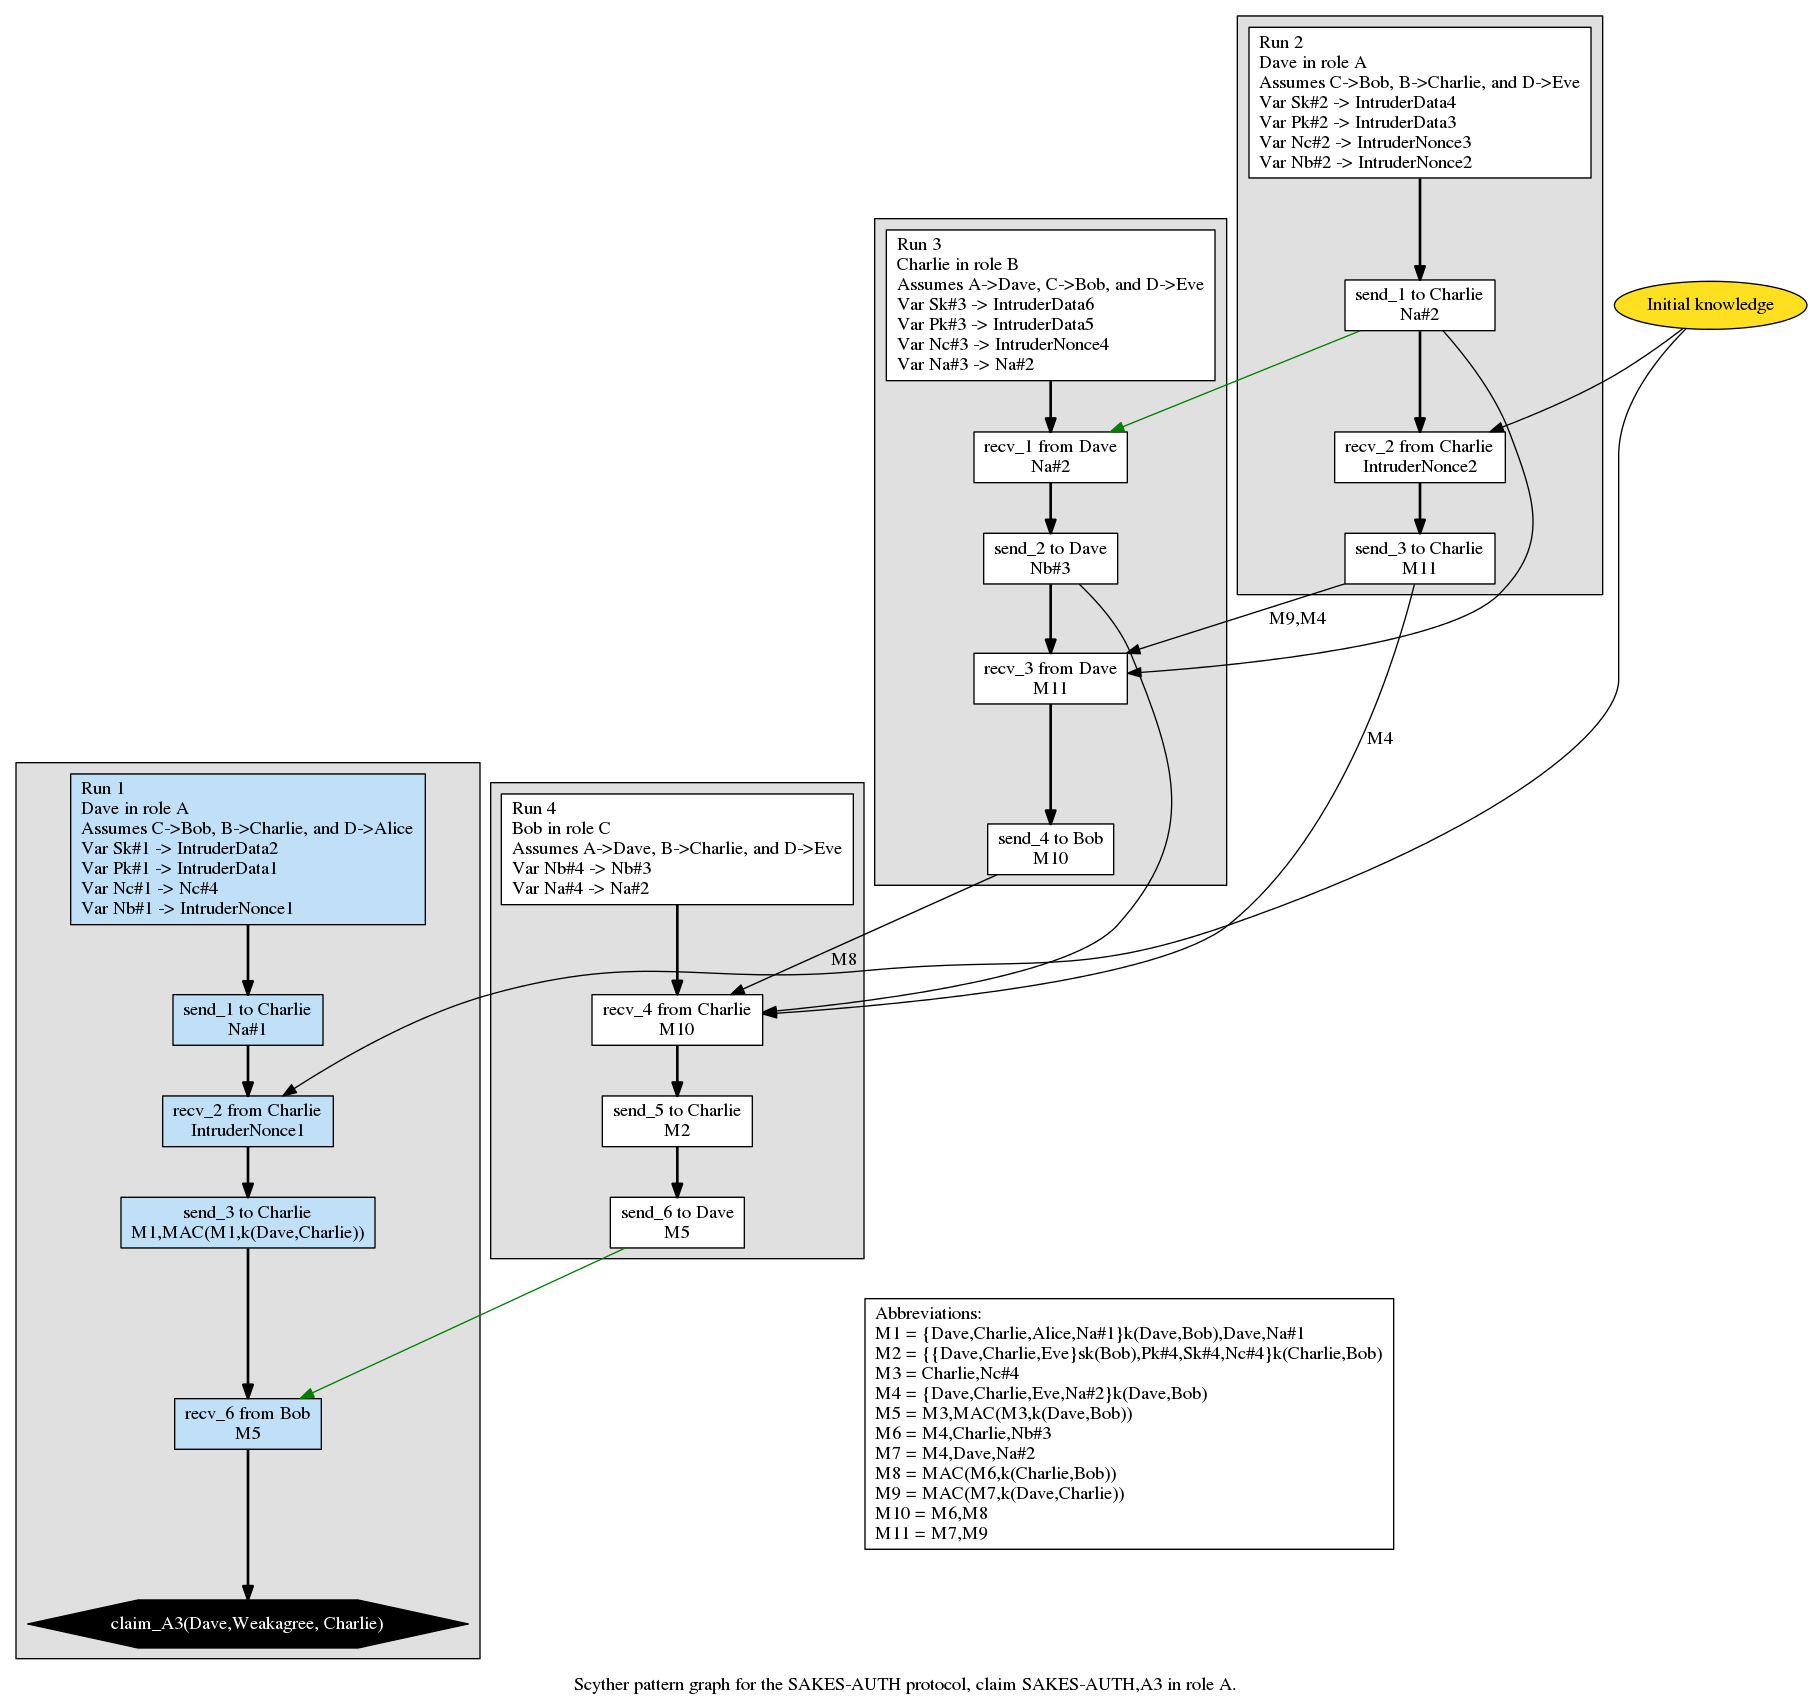
\includegraphics[scale=0.20]{attacks/sakes-auth-a-weakagree-attack2.png}
	\caption{Graph of the discovered attack on the weak agreement property of the role A in the authentication phase of SAKES.}
	\label{fig:sakes-attack-weakagree}
\end{sidewaysfigure}

\begin{sidewaysfigure}
	\centering
	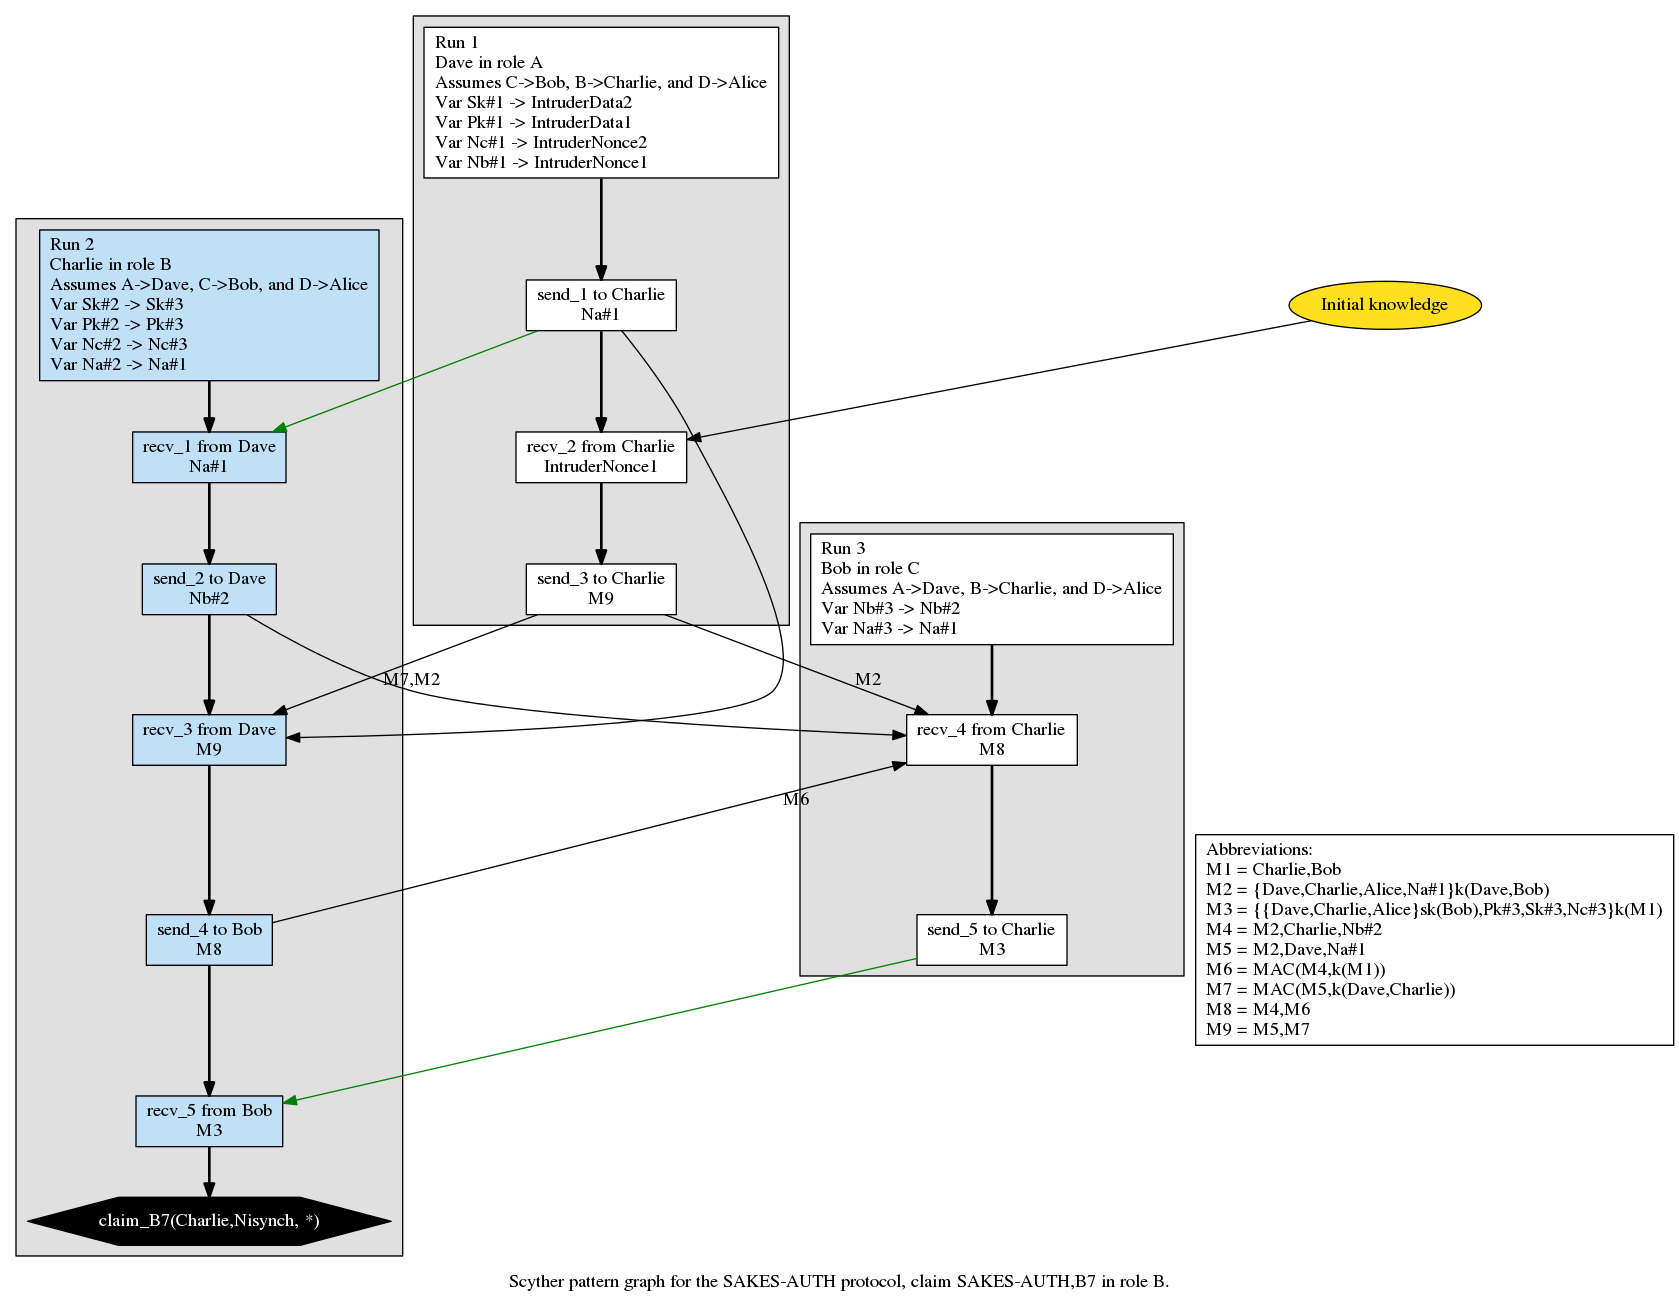
\includegraphics[scale=0.30]{attacks/sakes-auth-a-nisynch-attack2.png}
	\caption{Graph of the discovered attack on the Nisynch property of the roles A, B, and C from A's point of view in the authentication phase of SAKES.}
	\label{fig:sakes-attack-nisynch}
\end{sidewaysfigure}

\begin{sidewaysfigure}
	\centering
	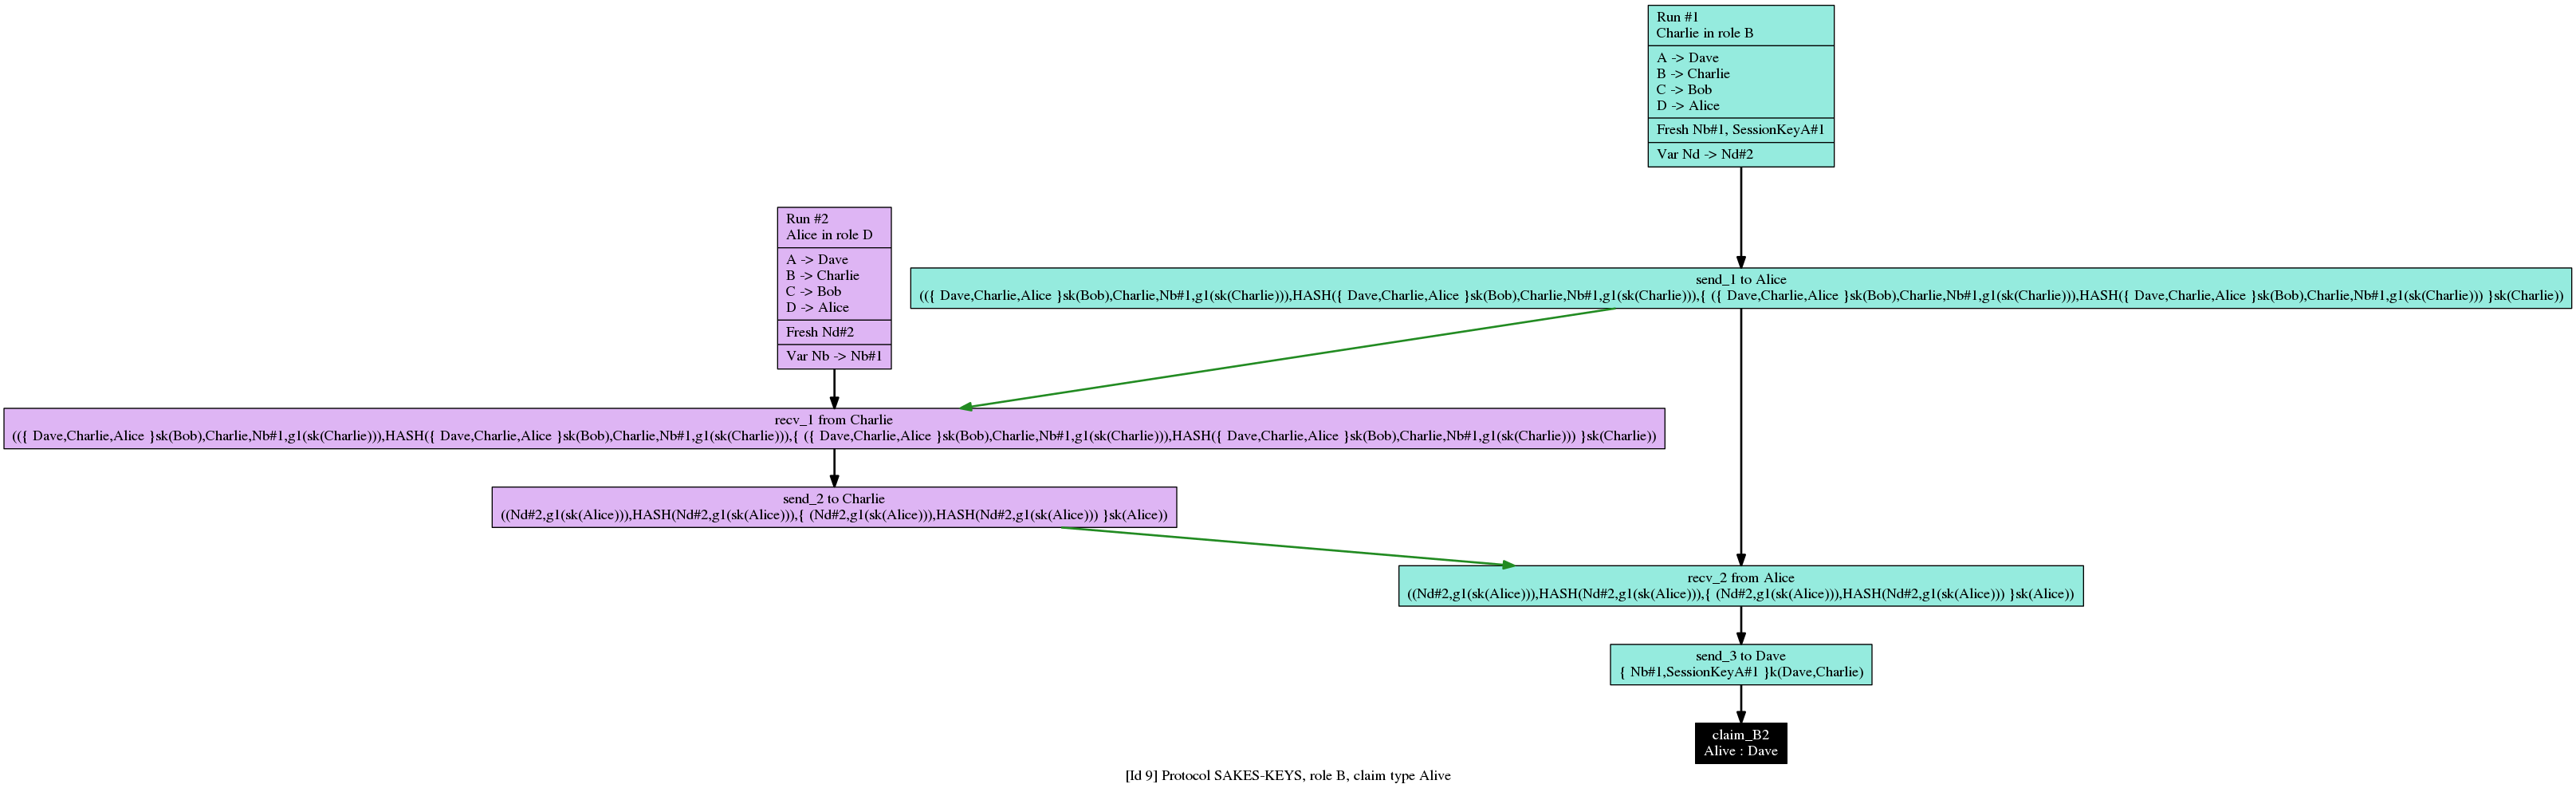
\includegraphics[scale=0.19]{attacks/sakes-keys-b-alive-a-attack.png}
	\caption{Graph of the discovered attack on the entity authentication of the end device in role B in the key establishment phase of SAKES.}
	\label{fig:sakes-attack-keys-b-alive-a}
\end{sidewaysfigure}

\begin{sidewaysfigure}
	\centering
	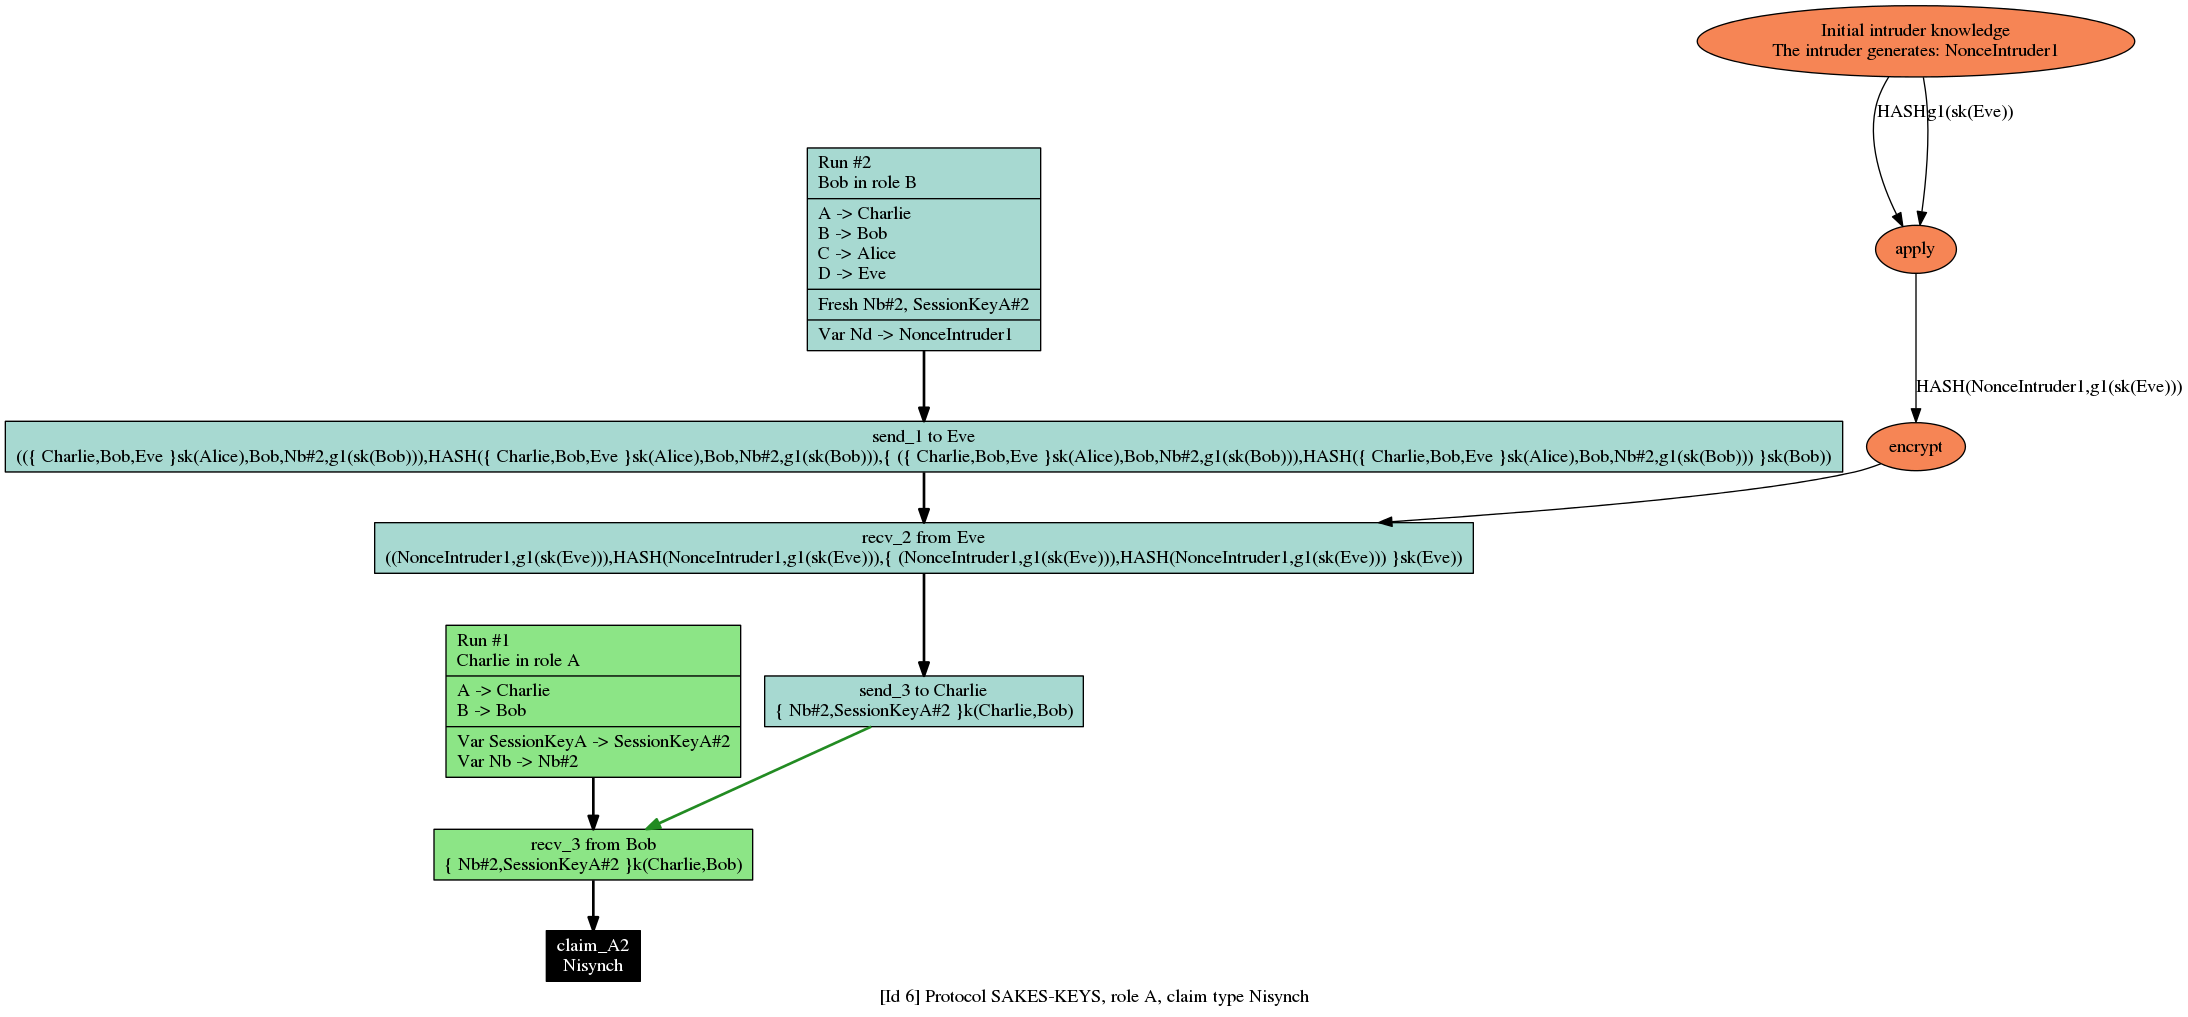
\includegraphics[scale=0.27]{attacks/sakes-keys-a-niagree-nisynch-attack.png}
	\caption{Graph of the discovered attack on the Niagree and Nisynch properties in the role A in the key establishment phase of SAKES.}
	\label{fig:sakes-attack-keys-a-niagree-nisynch}
\end{sidewaysfigure}

\begin{sidewaysfigure}
	\centering
	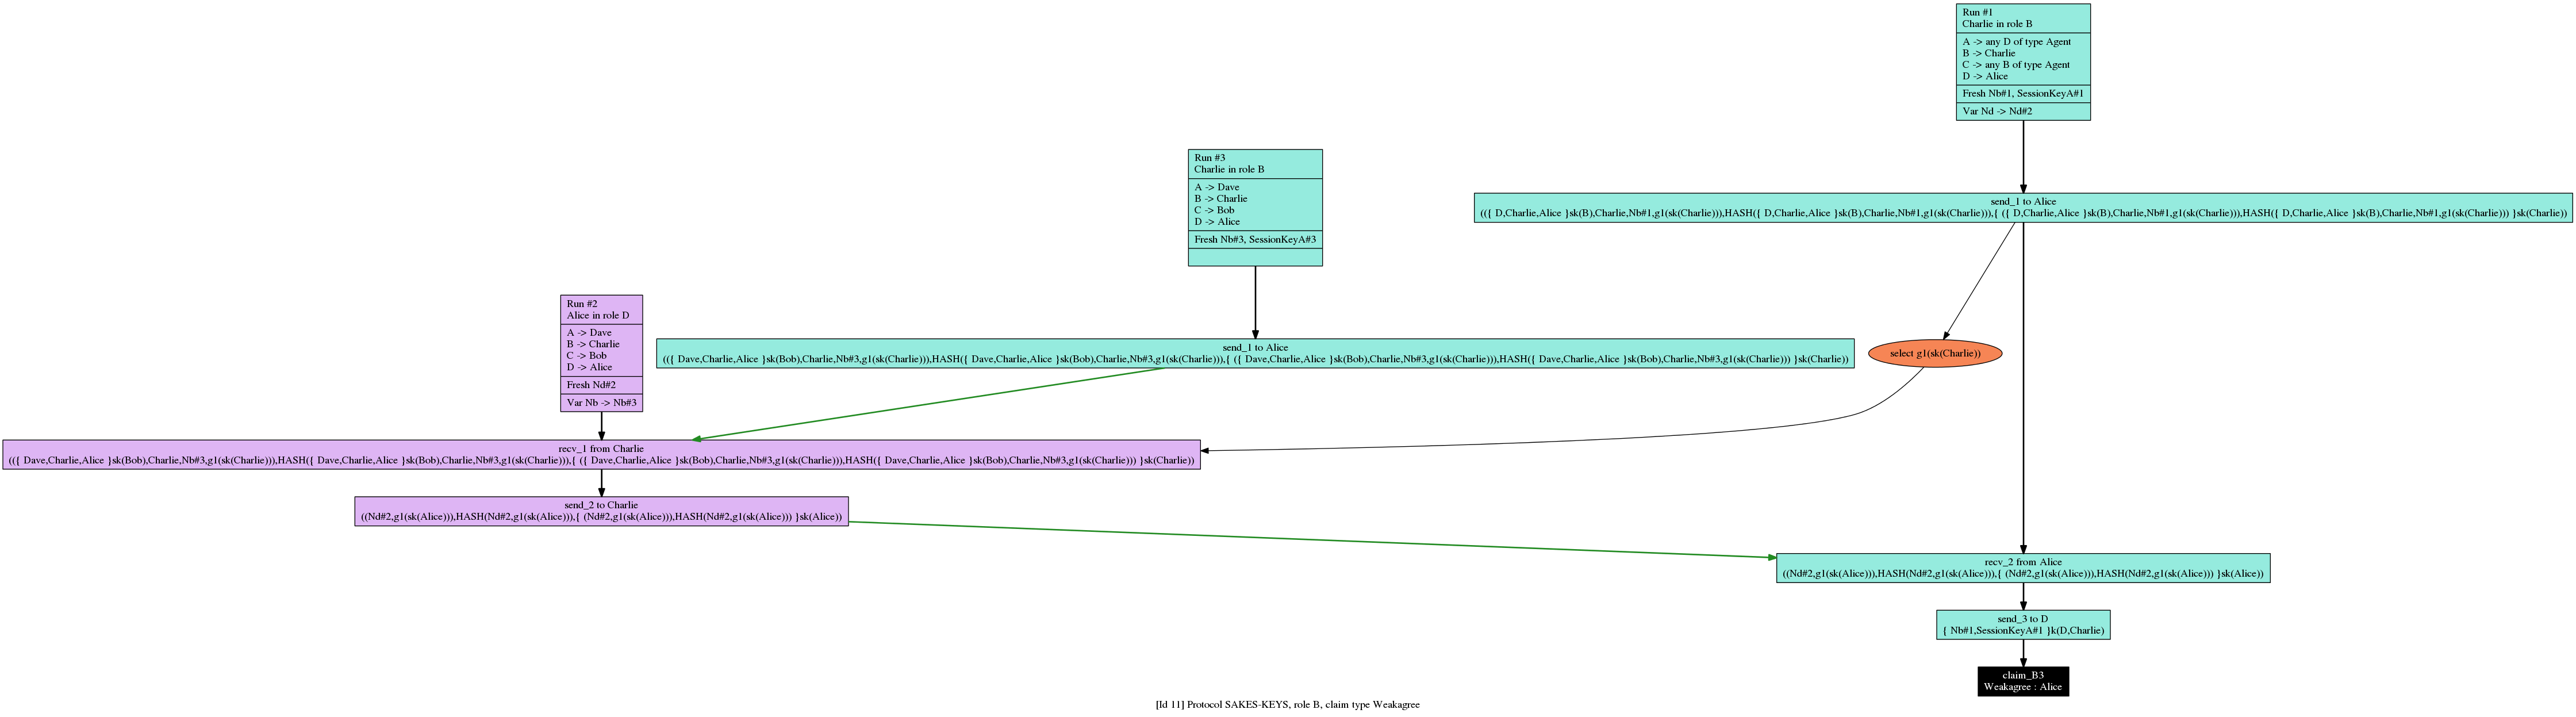
\includegraphics[scale=0.13]{attacks/sakes-keys-b-weakagree-d-attack.png}
	\caption{Graph of the discovered attack on the weak agreement property of D in role B in the key establishment phase of SAKES.}
	\label{fig:sakes-attack-keys-b-weakagree-d}
\end{sidewaysfigure}

\begin{sidewaysfigure}
	\centering
	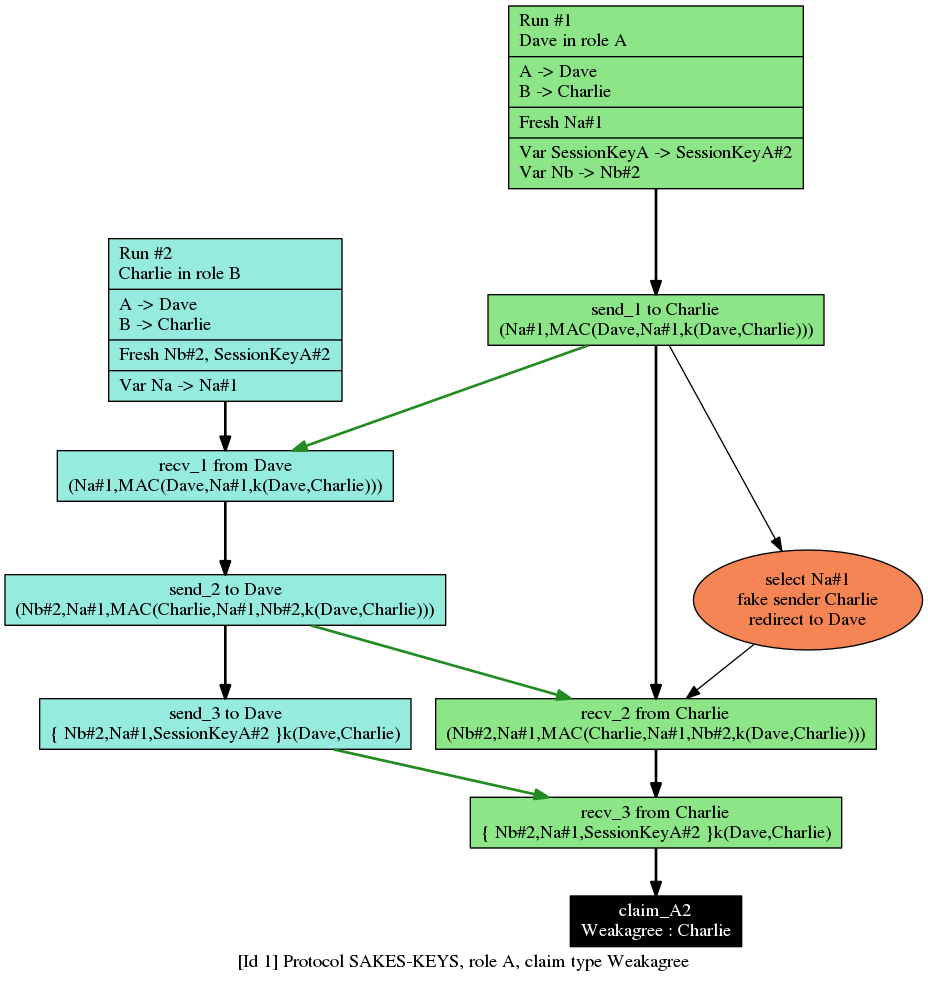
\includegraphics[scale=0.35]{attacks/sakes-keys-a-weakagree-b-attack.png}
	\caption{Graph of the discovered attack on the weak agreement property of B in role A in the key establishment phase of SAKES.}
	\label{fig:sakes-attack-keys-a-weakagree-b}
\end{sidewaysfigure}


\chapter{Notations}

\section{Notation}
\label{app:notations}

\begin{tcolorbox}[title=Notation used in protocol specifications]
\begin{tabular}{ll}
\multicolumn{1}{p{1.3cm}}{\textbf{Symbol}} & \multicolumn{1}{p{4cm}}{\textbf{Meaning}}\\
A, B, C, D & Nodes\ A, B, C, D\\
$\langle{\ ...\ }\rangle{}$ & Unauthenticated message\\
$\langle{\ ...\ }\rangle{k}$ & Authenticated message with key $k$\\
$\{\ ...\ \}_k$ & Message encrypted with key $k$\\
$A \rightarrow B$ & Message sent from A to B\\
$A \rightarrow *$ & Message broadcasted from A\\
$(Pk_{node}, Sk_{node})$ & Public key pair for a node \\
$ID_{node}$ & Identity of a node\\
$AES(k, m)$ & AES encryption of message $m$ with key $k$\\
$N_{node}$ & Cryptographic nonce generated by a node\\
$X\ ||\ Y$ & Concatenation of two terms X and Y\\ 
\end{tabular}
\end{tcolorbox}


